\documentclass[]{beamer}
%\documentclass[handout]{beamer}
%\usepackage[dvips]{color}
%\usepackage{beamerprosper}
\usepackage{graphicx}
%\usepackage{psfrag, pstricks}
\usepackage{amsmath,amssymb,array,comment,eucal}
\newcommand{\e}{\mathbf{e}}
\renewcommand{\P}{\mathbf{P}}
\newcommand{\F}{\mathbf{F}}
\newcommand{\R}{\textsf{R}}
\newcommand{\mat}[1] {\mathbf{#1}}
%\newcommand{\ind}{\mathrel{\mathop{\sim}\limits^{\mathit{ind}}}}
%\newcommand{\iid}{\mathrel{\mathop{\sim}\limits^{\mathit{iid}}}}
\newcommand{\E}{\textsf{E}}
\newcommand{\SE}{\textsf{SE}}
\newcommand{\SSE}{\textsf{SSE}}
\newcommand{\RSS}{\textsf{RSS}}
\newcommand{\FSS}{\textsf{FSS}}
\renewcommand{\SS}{\textsf{SS}}
\newcommand{\MSE}{\textsf{MSE}}
\newcommand{\SSR}{\textsf{SSR}}
\newcommand{\Be}{\textsf{Beta}}
\newcommand{\St}{\textsf{St}}
%\newcommand{\C}{\textsf{C}}
\newcommand{\GDP}{\textsf{GDP}}
\newcommand{\NcSt}{\textsf{NcSt}}
\newcommand{\Bin}{\textsf{Bin}}
\newcommand{\NB}{\textsf{NegBin}}
\renewcommand{\NG}{\textsf{NG}}
\newcommand{\N}{\textsf{N}}
\newcommand{\Ber}{\textsf{Ber}}
\newcommand{\Poi}{\text{Poi}}
\newcommand{\Gam}{\textsf{Gamma}}
\newcommand{\BB}{\textsf{BB}}
\newcommand{\Gm}{\textsf{G}}
\newcommand{\Un}{\textsf{Unif}}
\newcommand{\Ex}{\textsf{Exp}}
\newcommand{\DE}{\textsf{DE}}
\newcommand{\tr}{\textsf{tr}}
\newcommand{\cF}{{\cal{F}}}
\newcommand{\cL}{{\cal{L}}}
\newcommand{\cI}{{\cal{I}}}
\newcommand{\cB}{{\cal{B}}}
\newcommand{\cP}{{\cal{P}}}
\newcommand{\bbR}{\mathbb{R}}
\newcommand{\bbN}{\mathbb{N}}
\newcommand{\pperp}{\mathrel{{\rlap{$\,\perp$}\perp\,\,}}}
\newcommand{\OFP}{(\Omega,\cF, \P)}
\newcommand{\eps}{\boldsymbol{\epsilon}}
\newcommand{\1}{\mathbf{1}_n}
\newcommand{\gap}{\vspace{8mm}}
\newcommand{\ind}{\mathrel{\mathop{\sim}\limits^{\rm ind}}}
\newcommand{\simiid}{\ensuremath{\mathrel{\mathop{\sim}\limits^{\rm
iid}}}}
\newcommand{\eqindis}{\ensuremath{\mathrel{\mathop{=}\limits^{\rm D}}}}
\newcommand{\iid}{\textit{i.i.d.}}
\newcommand{\SSZ}{S_{zz}}
\newcommand{\SZW}{S_{zw}}
\newcommand{\Var}{\textsf{Var}}
\newcommand{\corr}{\textsf{corr}}
\newcommand{\diag}{\textsf{diag}}
\newcommand{\var}{\textsf{var}}
\newcommand{\Cov}{\textsf{Cov}}
\newcommand{\Sam}{{\cal S}}
\def\H{\mathbf{H}}
\newcommand{\I}{\mathbf{I}}
\newcommand{\Y}{\mathbf{Y}}
\newcommand{\tY}{\tilde{\mathbf{Y}}}
\newcommand{\Yhat}{\hat{\mathbf{Y}}}
\newcommand{\Yobs}{\mathbf{Y}_{{\cal S}}}
\newcommand{\barYobs}{\bar{Y}_{{\cal S}}}
\newcommand{\barYmiss}{\bar{Y}_{{\cal S}^c}}
\def\bv{\mathbf{b}}
\def\X{\mathbf{X}}
\def\tX{\tilde{\mathbf{X}}}
\def\x{\mathbf{x}}
\def\xbar{\bar{\mathbf{x}}}
\def\Xbar{\bar{\mathbf{X}}}
\def\Xg{\mathbf{X}_{\boldsymbol{\gamma}}}
\def\Ybar{\bar{\Y}}
\def\ybar{\bar{y}}
\def\y{\mathbf{y}}
\def\Yf{\mathbf{Y_f}}
\def\W{\mathbf{W}}
\def\L{\mathbf{L}}
\def\w{\mathbf{w}}
\def\U{\mathbf{U}}
\def\V{\mathbf{V}}
\def\Q{\mathbf{Q}}
\def\Z{\mathbf{Z}}
\def\z{\mathbf{z}}
\def\v{\mathbf{v}}
\def\u{\mathbf{u}}

\def\zero{\mathbf{0}}
\def\one{\mathbf{1}}
\newcommand{\taub}{\boldsymbol{\tau}}
\newcommand{\betav}{\boldsymbol{\beta}}
\newcommand{\alphav}{\boldsymbol{\alpha}}
\newcommand{\A}{\mathbf{A}}
\def\a{\mathbf{a}}
\def\K{\mathbf{K}}
\newcommand{\B}{\mathbf{B}}
\def\b{\boldsymbol{\beta}}
\def\bhat{\hat{\boldsymbol{\beta}}}
\def\btilde{\tilde{\boldsymbol{\beta}}}
\def\tb{\tilde{\boldsymbol{\beta}}}
\def\bg{\boldsymbol{\beta_\gamma}}
\def\bgnot{\boldsymbol{\beta_{(-\gamma)}}}
\def\mub{\boldsymbol{\mu}}
\def\tmub{\tilde{\boldsymbol{\mu}}}
\def\muhat{\hat{\boldsymbol{\mu}}}
\def\t{\boldsymbol{\theta}}
\def\tk{\boldsymbol{\theta}_k}
\def\tj{\boldsymbol{\theta}_j}
\def\Mk{\boldsymbol{{\cal M}}_k}
\def\M{\boldsymbol{{\cal M}}}
\def\Mj{\boldsymbol{{\cal M}}_j}
\def\Mi{\boldsymbol{{\cal M}}_i}
\def\Mg{{\boldsymbol{{\cal M}_\gamma}}}
\def\Mnull{\boldsymbol{{\cal M}}_{N}}
\def\gMPM{\boldsymbol{\gamma}_{\text{MPM}}}
\def\gHPM{\boldsymbol{\gamma}_{\text{HPM}}}
\def\Mfull{\boldsymbol{{\cal M}}_{F}}
\def\tg{\boldsymbol{\theta}_{\boldsymbol{\gamma}}}
\def\g{\boldsymbol{\gamma}}
\def\eg{\boldsymbol{\eta}_{\boldsymbol{\gamma}}}
\def\G{\mathbf{G}}
\def\cM{\cal M}
\def\D{\Delta}
\def \shat{{\hat{\sigma}}^2}
\def\uv{\mathbf{u}}
\def\l {\lambda}
\def\d{\delta}
\def\Sigmab{\boldsymbol{\Sigma}}
\def\Lambdab{\boldsymbol{\Lambda}}
\def\lambdab{\boldsymbol{\lambda}}
\def\Mg{{\cal M}_\gamma}
\def\S{{\cal{S}}}
\def\qg{p_{\boldsymbol{\gamma}}}
\def\pg{p_{\boldsymbol{\gamma}}}
\def\t{\boldsymbol{\theta}}  
\def\T{\boldsymbol{\Theta}}  
\usepackage{verbatim}
% abbreviation
\def\logit{\textsf{logit}}


\title{Introduction to Generalized Additive Models}

\date{\today}

\begin{document}
\maketitle
\begin{frame}[fragile]\frametitle{Beyond Linearity}
Wage data from Introduction to Statistical Learning

Residual plots from Simple Linear Regression of Wage on Age:
\centerline{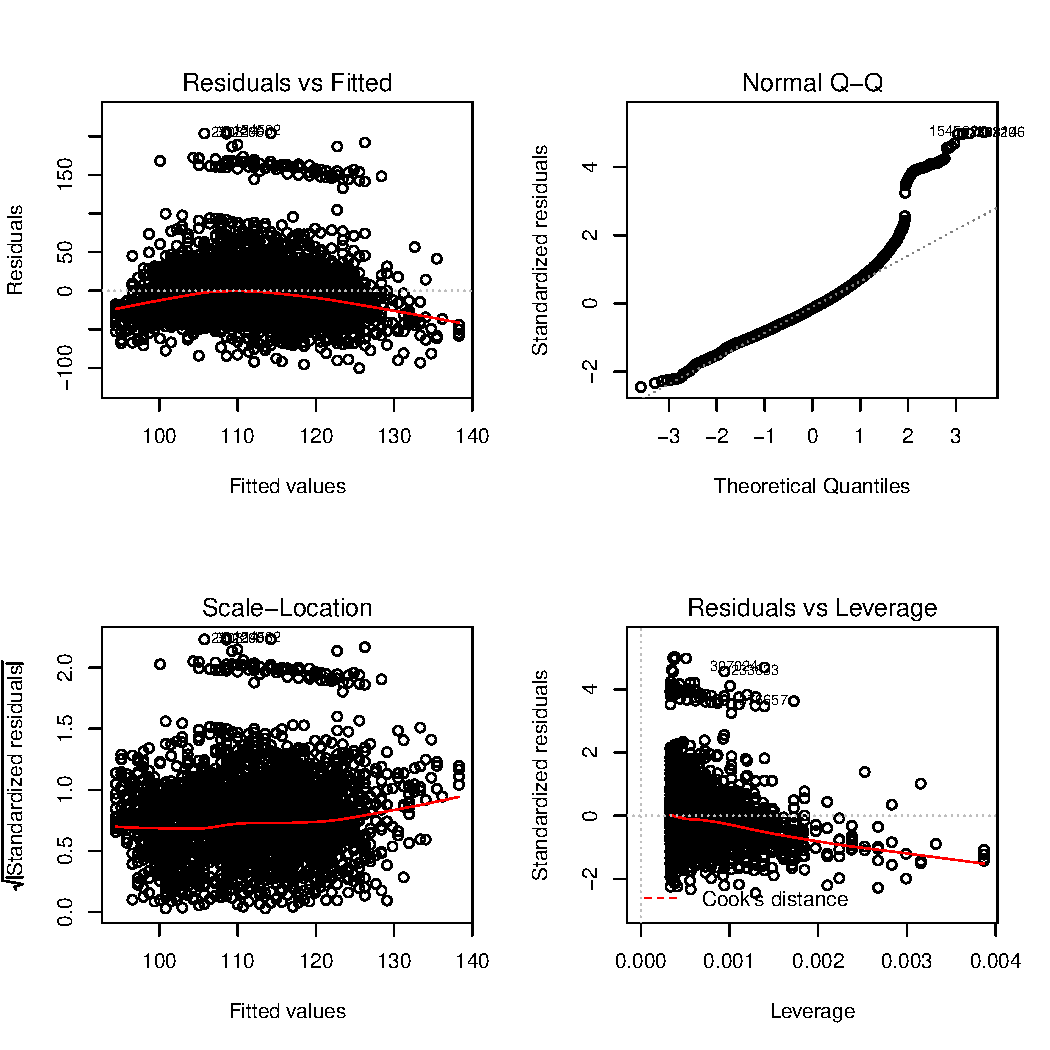
\includegraphics[height=3in]{resid-slr}}
\end{frame}

\begin{frame}[fragile]\frametitle{Polynomial Regression}
\begin{verbatim}
> summary(lm(wage ~ age + I(age^2) + I(age^3) + I(age^4), 
  data=Wage))
Coefficients:
              Estimate Std. Error t value Pr(>|t|)    
(Intercept) -1.842e+02  6.004e+01  -3.067 0.002180 ** 
age          2.125e+01  5.887e+00   3.609 0.000312 ***
I(age^2)    -5.639e-01  2.061e-01  -2.736 0.006261 ** 
I(age^3)     6.811e-03  3.066e-03   2.221 0.026398 *  
I(age^4)    -3.204e-05  1.641e-05  -1.952 0.051039 .  
---
Signif. codes:  0 ‘***’ 0.001 ‘**’ 0.01 ‘*’ 0.05 ‘.’ 0.1 ‘ ’ 1

Residual standard error: 39.91 on 2995 degrees of freedom
Multiple R-squared:  0.08626,	Adjusted R-squared:  0.08504 
F-statistic: 70.69 on 4 and 2995 DF,  p-value: < 2.2e-16
\end{verbatim}

\end{frame}
\begin{frame}[fragile]{Orthogonal Polynomial}
\begin{verbatim}
> summary(lm(wage ~ poly(age,4),data=Wage))

Coefficients:
               Estimate Std. Error t value Pr(>|t|)    
(Intercept)    111.7036     0.7287 153.283  < 2e-16 ***
poly(age, 4)1  447.0679    39.9148  11.201  < 2e-16 ***
poly(age, 4)2 -478.3158    39.9148 -11.983  < 2e-16 ***
poly(age, 4)3  125.5217    39.9148   3.145  0.00168 ** 
poly(age, 4)4  -77.9112    39.9148  -1.952  0.05104 .  
---

Residual standard error: 39.91 on 2995 degrees of freedom
Multiple R-squared:  0.08626,	Adjusted R-squared:  0.08504 
F-statistic: 70.69 on 4 and 2995 DF,  p-value: < 2.2e-16
\end{verbatim}
\end{frame}
\begin{frame}\frametitle{Fitted Values}
  \centerline{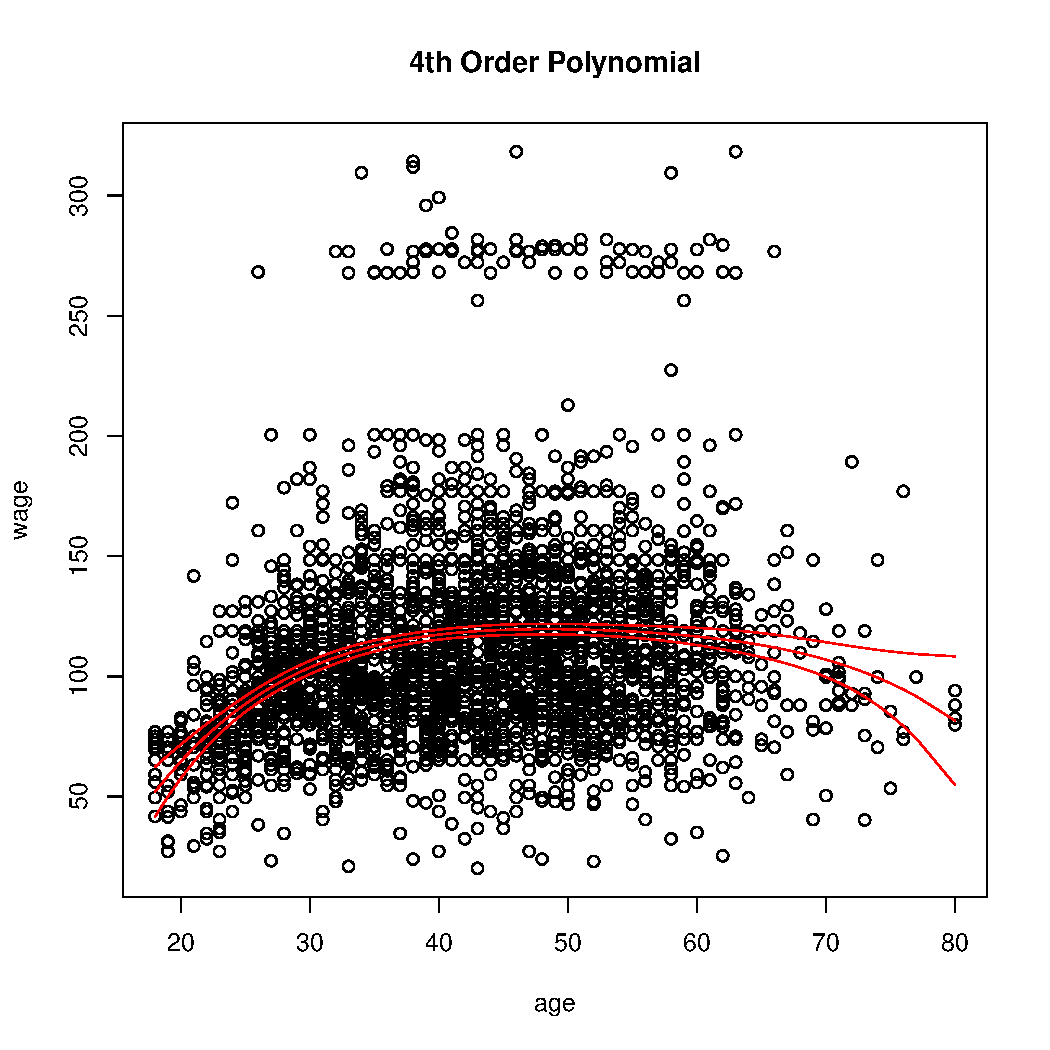
\includegraphics[height=3in]{poly}}
\end{frame}

\begin{frame}\frametitle{Problems}
  \begin{itemize}
  \item Higher order terms may be needed to fit data globally \pause
  \item generally do not go above 3rd order or 4th order polynomial -
        may be too flexible \pause
  \item fit piece-wise polynomials over different ranges \pause
  \item is function continuous where they join? \pause
  \item is function differentiable where they join? \pause 
  \end{itemize}
Add constraints - lose degrees of freedom
\end{frame}

\begin{frame}\frametitle{Piecewise Polynomials}

\centerline{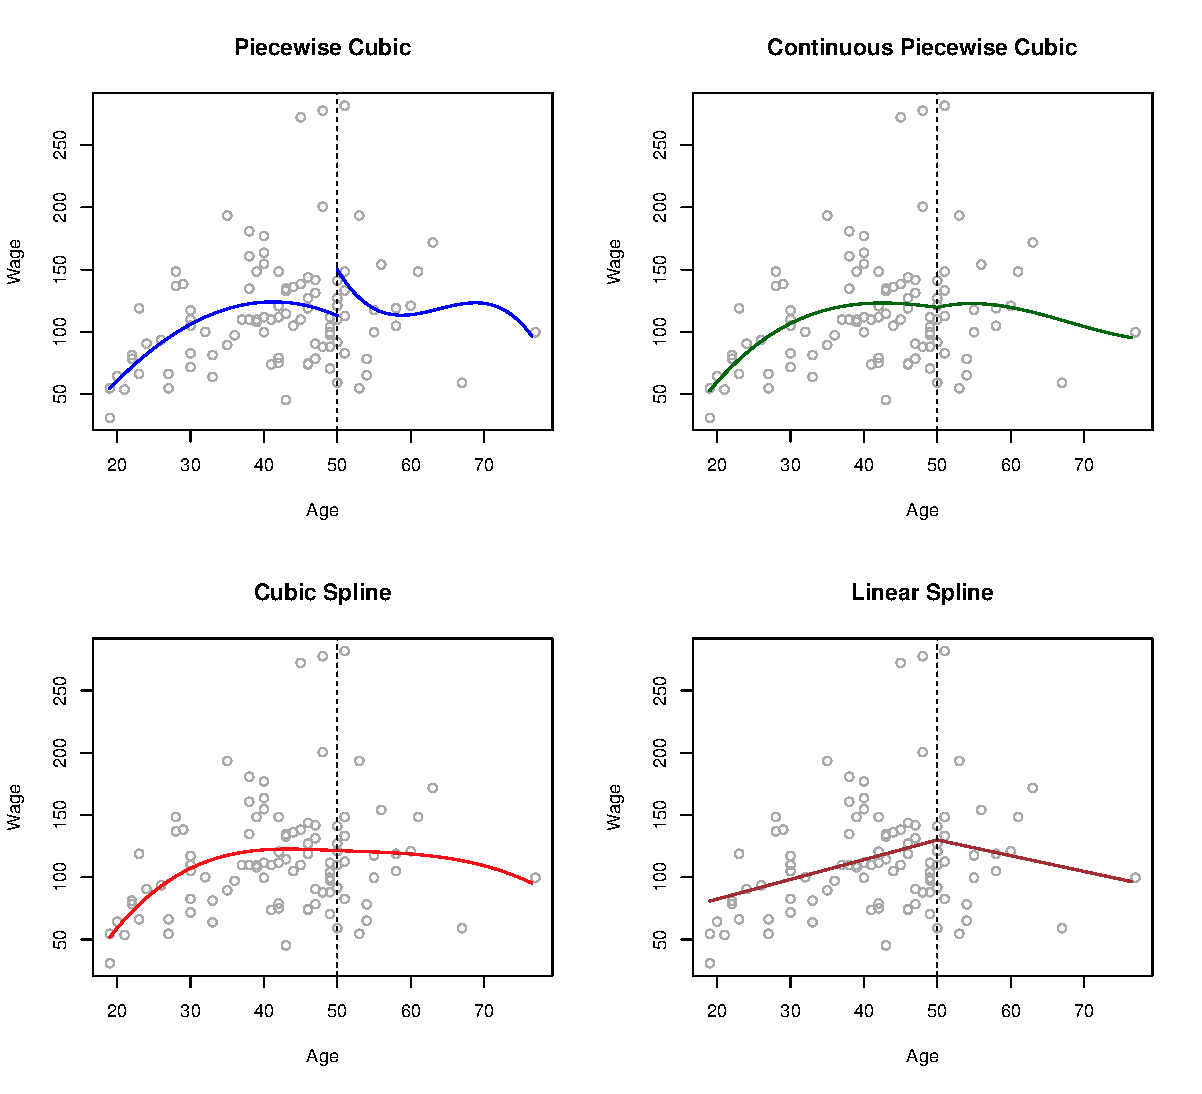
\includegraphics[height=3in]{7-3}}

\end{frame}
\begin{frame}\frametitle{Spline Basis}
Alternative way to represent the model so that we have continuity, continuous first and
second derivatives  is 
$$Y_i = \beta_0 + \beta_1 x_i + \beta_2 x_1^2 + \beta_3 x_i^3 + h(x_i,\xi) \beta_4 + \epsilon_i$$

where $\xi$ is a ``knot''' in a truncated cubic basis function
$$
h(x_i, \xi) \equiv (x_i - \xi)^3_+ =  \left\{
\begin{array}{ll}
  (x_i - \xi)^3 & \text{ if }  x_i > \xi \\
  0 & \text{ otherwise} 
\end{array} \right.
$$\pause

We can add additional terms that each with 1 degree of freedom
$$Y_i = \beta_0 + \beta_1 x_i + \beta_2 x_1^2 + \beta_3 x_i^3 +
\sum_{k=1}^{K}h(x_i,\xi_k) \alpha_{k} + \epsilon_i$$ \pause


\end{frame}

\begin{frame}\frametitle{Splines}

  \begin{itemize}
  \item B-splines  (reduces multicollinearity between terms from
    truncated basis) {\tt splines} package in R to use {\tt bs(x)} to
    construct basis \pause
  \item natural splines   (add more constraints so that function is linear
    outside range of data) \pause
\item smoothing splines \pause
  \end{itemize}

Choice of knots and/or degrees of freedom? \pause   Smoothing splines place
a knot at each data point, but adds
 a penalty to prevent over-fitting:

$$ \sum (Y_i - g(x_i))^2 +  \lambda \int g^{"}(t)^2 \, dt $$
\pause
This can be reformulated as a Bayesian model with a Gaussian g-prior.
packages use LOOCV or GCV to choose $\lambda$

Simon Wood's package mgcv in R   and book ``Generalized Additive Models: An Introduction with R''


\end{frame}

\begin{frame}[fragile]\frametitle{Fitting GAMs in R}
\begin{verbatim}
> library(mgcv)
> wage.gam = gam(wage ~ s(age), data=Wage)
> summary(wage.gam)
Parametric coefficients:
            Estimate Std. Error t value Pr(>|t|)    
(Intercept) 111.7036     0.7282   153.4   <2e-16 ***

Approximate significance of smooth terms:
         edf Ref.df     F p-value    
s(age) 5.298  6.399 44.34  <2e-16 ***
---
Signif. codes:  0 ‘***’ 0.001 ‘**’ 0.01 ‘*’ 0.05 ‘.’ 0.1 ‘ ’ 1

R-sq.(adj) =  0.0864   Deviance explained =  8.8%
GCV = 1594.2  Scale est. = 1590.9    n = 3000
\end{verbatim}
\end{frame}
\begin{frame}\frametitle{Fitted Curve}
  plot(wage.gam)
\centerline{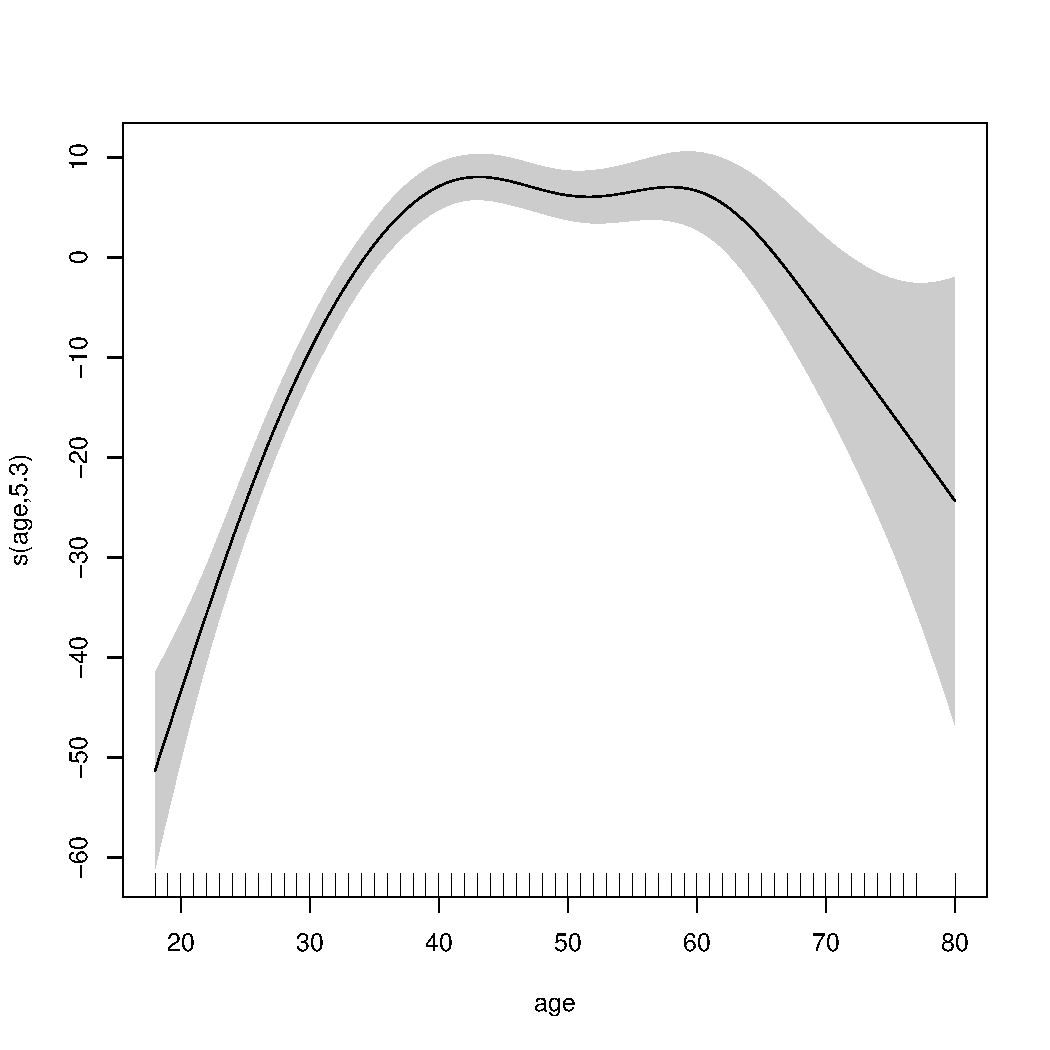
\includegraphics[height=3in]{gam-age}}
\end{frame}

\begin{frame}[fragile]\frametitle{More terms}
\begin{verbatim}
> wage.gam2 = gam(wage ~ s(year,k=7) + s(age), data=Wage)
> summary(wage.gam2)

Parametric coefficients:
            Estimate Std. Error t value Pr(>|t|)    
(Intercept) 111.7036     0.7266   153.7   <2e-16 ***
---

Approximate significance of smooth terms:
          edf Ref.df     F  p-value    
s(year) 1.000  1.000 14.18 0.000169 ***
s(age)  5.462  6.568 43.37  < 2e-16 ***

R-sq.(adj) =  0.0905   Deviance explained = 9.24%
GCV = 1587.7  Scale est. = 1583.7    n = 3000
\end{verbatim}
\end{frame}
\begin{frame}\frametitle{Year and Age Smooth fits}
  \centerline{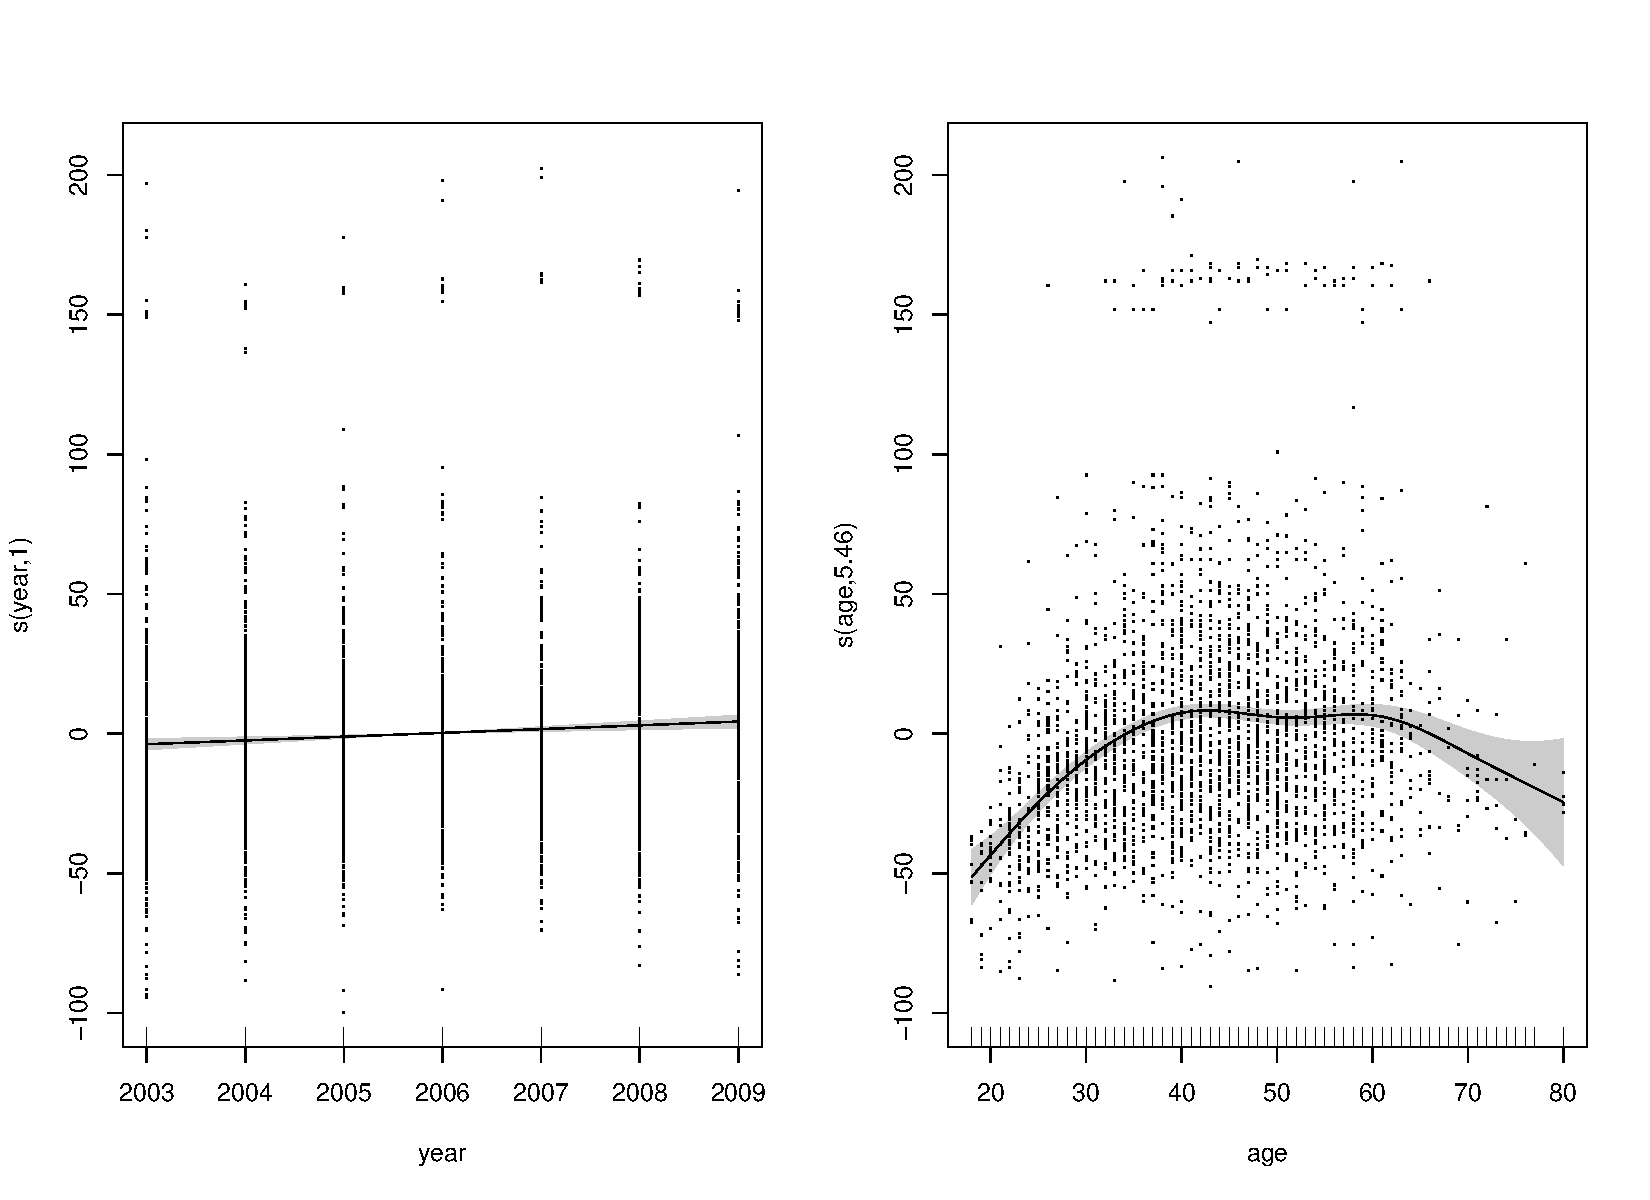
\includegraphics[height=3in]{gam-age-year}}
\end{frame}

\begin{frame}[fragile]\frametitle{Showing Factors}
\begin{verbatim}
wage.gam3 = gam(wage ~ s(year,k=7) + s(age) + education, data=Wage)
termplot(wage.gam3, se=T, rug=T, ask=F, col.se=2)
\end{verbatim}
\centerline{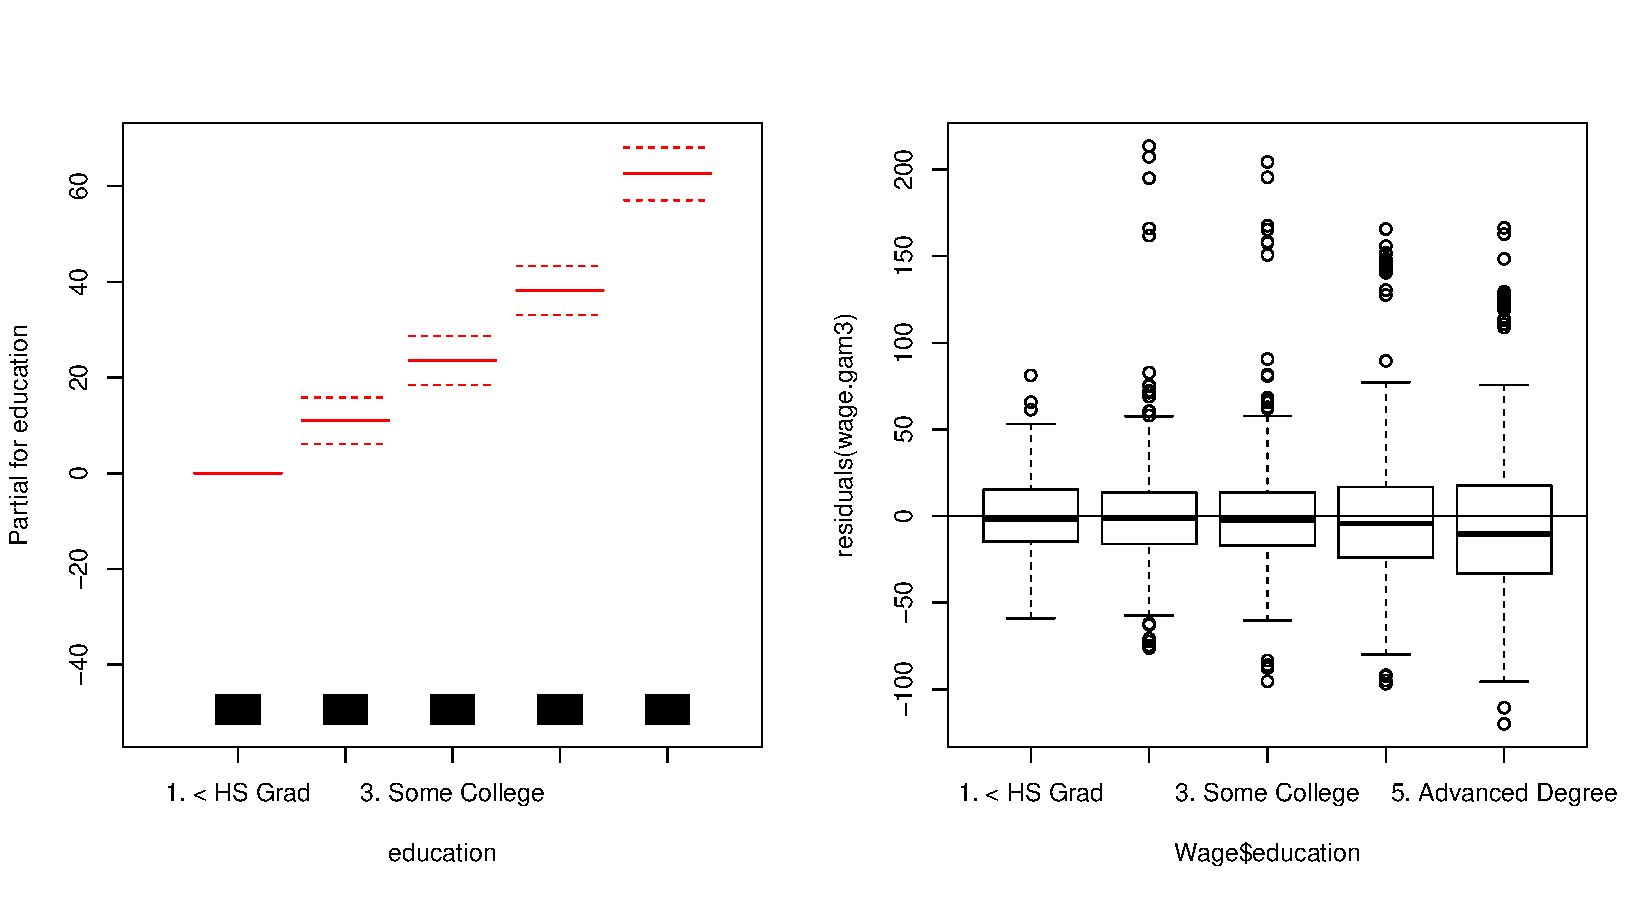
\includegraphics[height=2.5in]{edu-term}}
\end{frame}


\begin{frame}[fragile] \frametitle{Transformation + interaction}
\begin{verbatim}
wage.gam4 = gam(log(wage) ~ s(year,k=7) + 
s(age,education, bs="fs"), data=Wage)
\end{verbatim}
\centerline{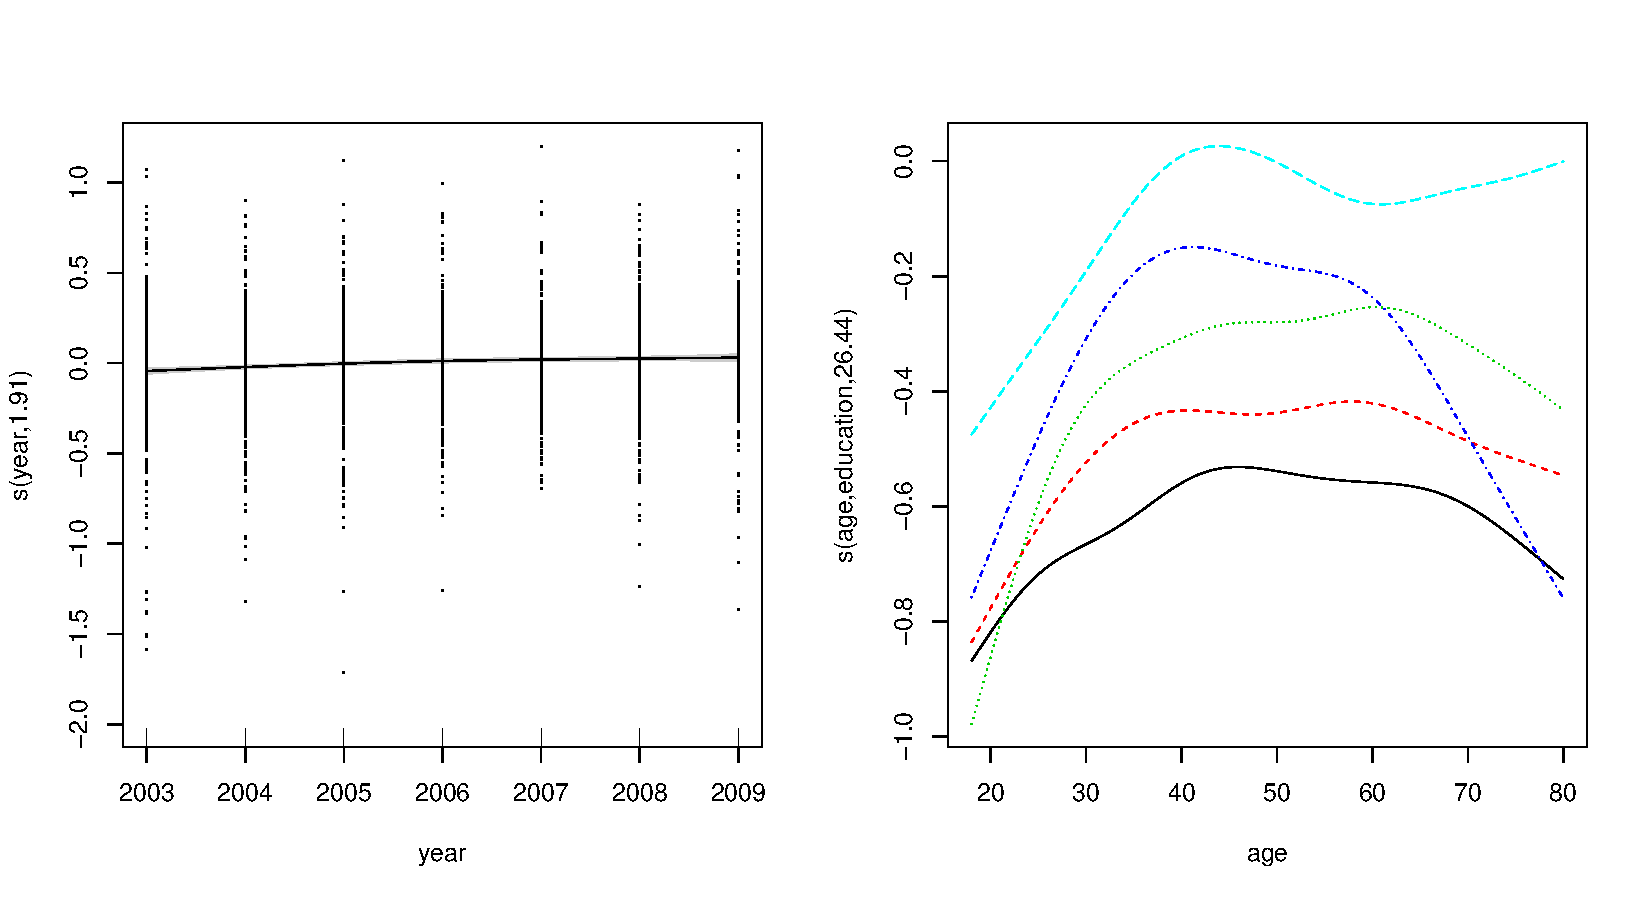
\includegraphics[height=2.5in]{wage-int}}
\end{frame}

\begin{frame} \frametitle{Residuals}
  \centerline{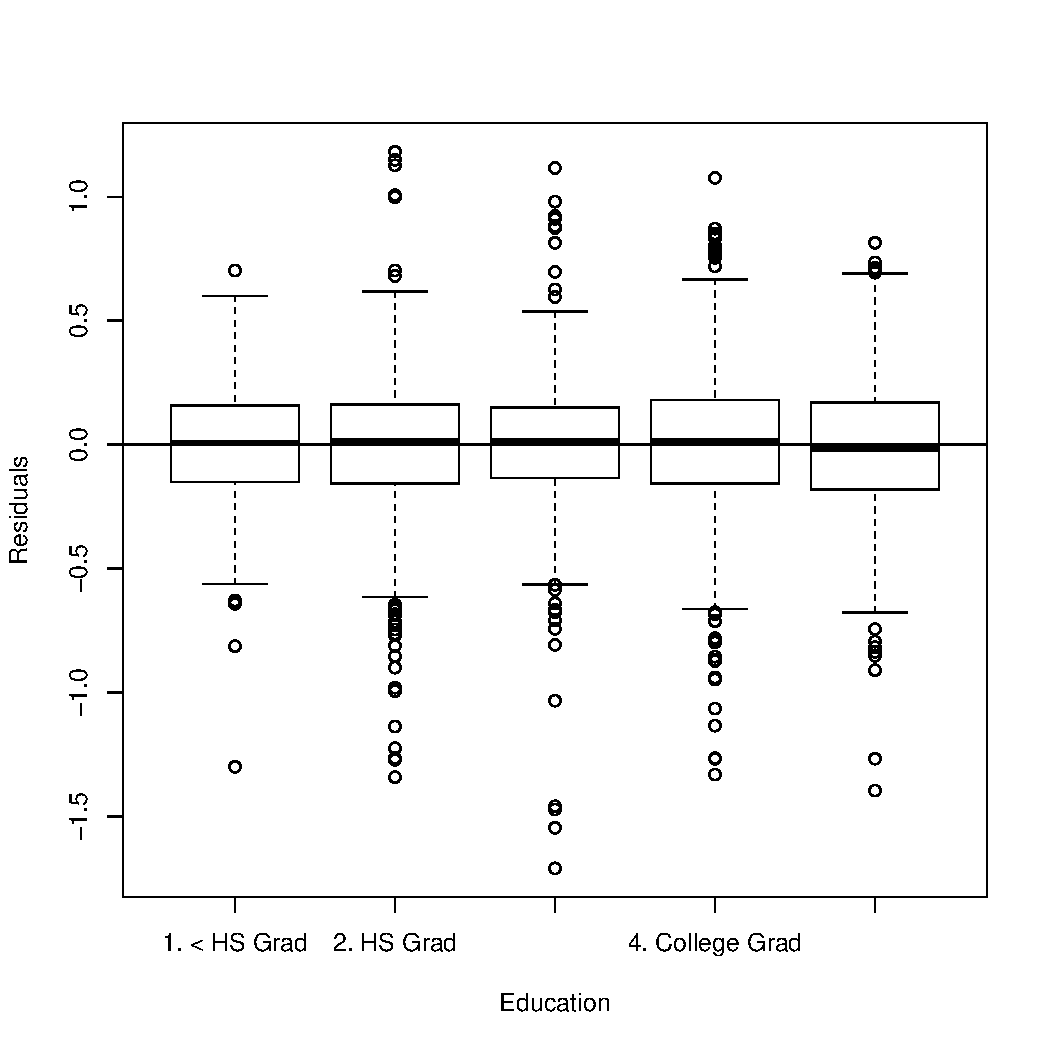
\includegraphics[height=2.5in]{resid-wage4}}
\end{frame}

\begin{frame}\frametitle{Summary}
  \begin{itemize}
  \item Over-fitting?   Choice of knots/df?
  \item Splits of data for model training/validation
  \item Other Variables
  \item Choice of Transformation?   (Box-Cox?)
  \end{itemize}

HW
\end{frame}
\end{document}